\chapter{Distributed Resolver Agents}\label{sec:resolver-agents}

\section{Overview}

Executing Software Composition Analysis (SCA) scans in \cxone will gather results
by analyzing packages found in the dependency tree for the code submitted for scan.  
The \cxone SCA scan first obtains a dependency tree, then performs an analysis
of the packages found in the dependency tree. The dependency
tree is obtained by executing the same build tools normally used to develop and produce a
distributable software package.  This execution is performed using two methods: server-side 
dependency tree resolution and client-side dependency tree resolution with \scaresolver.

The purpose of the distributed resolver agent configuration with \cxoneflow is to execute a
client-side dependency tree resolution in response to a source control event.  The \cxone
\intlink{sec:overview}{scan workflow} introduces the concept of a deferred scan which delegates
a scan with \scaresolver to an appropriate distributed resolver agent instance.  The selection of
the distributed resolver agent instance is performed through a tag configuration.

The basic workflow used by \cxoneflow with distributed resolver agents is as follows:

\begin{enumerate}
  \item The SCM event is received by \cxoneflow.  If the event \intlink{sec:overview}{qualifies to invoke} a scan and
    the \intlink{sec:resolver-elements}{resolver elements} in the \cxoneflow configuration exist, \cxoneflow attempts to select
    a distributed resolver agent tag. 
  \item The \cxone project is checked for a tag matching the configured \intlink{sec:yaml-resolver-resolver-tag-key}{resolver-tag-key}.
    If the project has a tag with the matching key and the value matches one of the values in the \intlink{sec:yaml-resolver-allowed-agent-tags}{allowed-agent-tags}
    configuration, that value is selected as the distributed resolver agent's tag.
  \item If the \cxone project does not have a tag with the matching \intlink{sec:yaml-resolver-resolver-tag-key}{resolver-tag-key} and
    \intlink{sec:yaml-resolver-default-agent-tag}{default-agent-tag} is configured, the default tag is selected as the the distributed resolver agent's tag.
  \item If a distributed resolver agent tag is selected, a request for a resolver scan is sent to distributed resolver agents having the selected tag.  The
    \cxone scan is deferred until the distributed resolver agent finishes a scan.
  \item Upon notification that a distributed resolver agent has finished the resolver scan, a \cxone scan is invoked.  A tag is added to the scan
    with the key value configured in the \intlink{sec:yaml-resolver-resolver-tag-key}{resolver-tag-key} element that indicates \textbf{success} or
    \textbf{failure} of the distributed resolver agent scan.
\end{enumerate}


\subsection{Server-Side Dependency Tree Resolution}

The dependency analysis for the code submitted to \cxone is performed
in the server-side \cxone environment by executing the package managers that match the composition of the code
under scan.  This generally works sufficiently when the code references only publicly-available, open-source
packages and is compatible with the package manager tooling installed in the \cxone environment.  

Not all software is composed of only publicly available packages nor does it always use package manager tooling
that is compatible with those installed in the \cxone environment.  Incompatibilities usually manifest
when some of the following issues are observed:

\begin{itemize}
  \item The dependency tree is incomplete when software references a private package repository.
  \item The dependency tree is incomplete when the code under scan is incompatible with the 
  package manager tools installed in the \cxone environment.
\end{itemize}

If the server-side dependency resolution is not producing accurate results, the general solution is to
perform a client-side dependency tree resolution with \scaresolver. 

\subsection{Client-Side Dependency Tree Resolution with \scaresolvertext}

The \scaresolver is typically scripted to execute in
a pipeline prior to the scan submission to \cxone.  This performs the dependency resolution
in the same environment as the code builds, which will generally resolve any tooling compatibility or network connection
problems.  

Since \cxoneflow is primarily driven by asynchronous web hook events and does not invoke a pipeline
where dependency resolution can be scripted, the distributed resolver agents can perform the dependency resolution using
\scaresolver. The diagram in Figure \ref{fig:resolver-agent-diagram} shows a typical deployment of the resolver agent.  


The resolver agent is deployed such that it can execute the same build tooling as is executed during the build
in a CI/CD pipeline. The \cxoneflow server delegates \scaresolver execution to the resolver agent to perform the dependency tree
resolution; this technique is similar to how a CI/CD pipeline delegates build script execution to a system with the correct
build environment.  The build execution is sometimes performed on a self-hosted "runner" agent or executed using a container with a specified tag. 

This execution delegation technique typically results in execution of the build tools that are appropriately
configured for the normal build.  The typical CI/CD pipeline runner will also have the correct network connection paths
needed to communicate to private package repositories.


\begin{figure}[ht]
  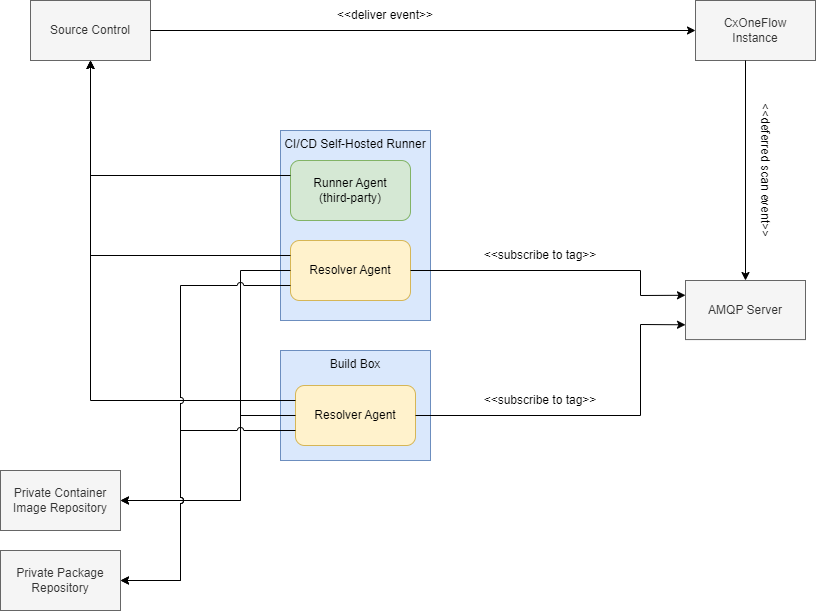
\includegraphics[width=\textwidth]{graphics/cxoneflow-diagrams-Resolver Agent Diagram.png}
  \caption{Resolver Agent Deployment Diagram}
  \label{fig:resolver-agent-diagram}
\end{figure}


\section{Distributed Resolver Security Considerations}\label{sec:dist-resolver-security-considerations}

Performing code builds, as is typically performed in a CI/CD pipeline, often includes
a bit of risk in that a build requires the execution of scripting.  There are often
controls in place to prevent anyone other than trusted authors from authoring those scripts.
As part of the scripts, there are often sensitive values exposed to the build script
for purposes of executing the build.

The use of distributed resolver agents involves some of the same risks as those that exist in
CI/CD pipeline builds.  To acquire a dependency tree of a project, the build tools
need to execute against the build definition to minimally produce the dependency
tree that is captured for the scan.  This action in itself can cause code to execute
as part of how the build definition is used by the tooling.  Some build tools allow
the dependencies themselves to execute code as part of the dependency resolution.
These dependencies, in some cases, can land malware in or exfiltrate data from the
environment where the dependency tree is compiled.

The \cxoneflow endpoint server itself does not invoke the build tools; this action is
delegated to the distributed resolver agents.  However, a required step of the
distributed resolver agent is to obtain a clone of the code for scanning.  To facilitate this,
the \cxoneflow endpoint server does send encoded SCM credentials to authorized
distributed resolver agents.  Section \ref{sec:resolver-agent-security} has more details
about security considerations for the distributed resolver agent.

Since the purpose of the resolver scan is to detect vulnerable and malicious packages,
it should be anticipated that malicious packages may be inadvertently referenced
by developers.  While the deployment recommendations of the distributed resolver agents
will help minimize exposure, the following security recommendations should be considered
as part of deployment of \cxoneflow with distributed resolver agents:

\begin{itemize}
  \item Use SSL for all message queue connections.
  \item Use SSL connections for delivering SCM events to the \cxoneflow endpoints.
  \item Isolate the distributed resolver agent either through installing on physically isolated machines or
  using OS permissions to isolate the distributed resolver agent runtime.
  \item Configure distributed resolver agents to execute build tools inside containers to isolate the build runtime from
  the distributed resolver agent runtime.
  \item If a scan detects a malware package, rotate all credentials used by \cxoneflow and distributed resolver agents
  after the malware is removed from the source code.
\end{itemize}

\section{Server Configuration for Distributed Resolver Agents}\label{sec:resolver-server}

Implementing the distributed resolver agents requires an AMQP message queue server that
is used for communication between the \cxoneflow server and the distributed resolver
agents.  Details about the message queue deployment can be found in Section \ref{sec:external-mq}.

\subsection{\cxoneflow Endpoint Configuration}

The endpoint server \hyperref[sec:yaml-config]{YAML configuration} will not utilize resolver agents
by default.  Using resolver agents requires a public/private key pair; the private key is configured
for use on the \cxoneflow endpoint and the public key is distributed with each resolver agent.  Before
configuring the use of distributed resolver agents, it is recommended to read about the security
concepts in Section \ref{sec:resolver-agent-security}.

The \cxoneflow endpoint will send messages signed by the private key to the distributed resolver
agents using the message queue.  The distributed resolver agents will validate the signature
using the public key; if the signature is not valid, the resolver agents will reject the message.

Distributed agents are identified using agent tags.  The \cxoneflow endpoint is configured by the
administrator with a list of allowed tags to prevent arbitrary agents from appearing.  The
server-side tag configuration is also used to set up the communication with the agents via
the message queue.  Anyone who installs a resolver agent must configure it to respond to messages
targeting at least one valid agent tag.


\subsubsection{Generating a Public/Private Key Pair}\label{ref:server-key-pair}

There are many ways to generate a public/private key pair.  There are only a few requirements
for key pairs produced by any method:

\begin{itemize}
  \item The private key must be unencrypted.
  \item Both the private and public key files must be PEM encoded.
  \item The public/private key algorithm is supported by the install Python \texttt{cryptography} library.
    As of this release, these algorithms have been tested:
  \begin{itemize}
      \item RSA 4096-bit
      \item ECDSA secp256k1
  \end{itemize}
\end{itemize}

One easy method of generating a public/private key pair is to use OpenSSL.  To generate an ECDSA public/private key pair,
the following command can be used.  The command will create the file \texttt{ec-priv.pem} that holds the unencrypted private key
and the file \texttt{ec-pub.pem} that holds the public key.

\begin{code}{OpenSSL Public/Private Key Creation}{[ECDSA]}{}
openssl ecparam -name secp256k1 -genkey -noout | tee ec-priv.pem | openssl ec -pubout > ec-pub.pem  
\end{code}

To generate an RSA 4096-bit public/private key pair,
the following command can be used.  The command will create the file \texttt{rsa-priv.pem} that holds the unencrypted private key
and the file \texttt{rsa-pub.pem} that holds the public key.

\begin{code}{OpenSSL Public/Private Key Creation}{[RSA]}{}
openssl genrsa 4096 |tee rsa-priv.pem | openssl rsa -pubout > rsa-pub.pem
\end{code}

The private key file may be stored as a secret referenced in the configuration YAML element \hyperref[sec:yaml-resolver-private-key]{resolver->private-key}.

\subsubsection{Resolver YAML Configuration}\label{sec:resolver-yaml-config}
The following YAML examples show a configuration for resolver agents with a list of allowed tags.
Some of the things to note in these examples:

\begin{itemize}
  \item The AMQP URL is stored as a secret since it contains credentials.
  \item The AMQP connection is common in both the \texttt{feedback} and \texttt{resolver} configuration.  This
  means the feedback workflows are using the same external message queue as the resolver.
\end{itemize}


\begin{code}{Minimal Resolver YAML Configuration Example}{[BitBucket Data Center]}{}
  secret-root-path: /run/secrets
  server-base-url: https://cxoneflow.mydomain.com:8443/

  amqp: &all-amqp
    amqp-url: amqp-server-credentials-secret

  bbdc:
      - service-name: BB
        repo-match: ^http(s)?:(\/){2}bitbucket\.corp\.com.*
        resolver:
          <<: *all-amqp
          private-key: resolver-agent-private-ec-key
          allowed-agent-tags:
            - thundercats
            - care-bears
            - galaxy-rangers
        feedback:
          <<: *all-amqp
          pull-request:
            enabled: True
        connection:
          base-url: https://bitbucket.corp.com
          shared-secret: scm-shared-secret
          api-auth:
            token: scm-token-secret
        cxone:
          tenant: mytenant
          oauth:
            client-id: my-oauth-id
            client-secret: my-oauth-secret
          iam-endpoint: US
          api-endpoint: US
\end{code}
  


\begin{code}{Minimal Resolver YAML Configuration Example}{[GitHub Enterprise]}{}
  secret-root-path: /run/secrets
  server-base-url: https://cxoneflow.mydomain.com:8443/

  amqp: &all-amqp
    amqp-url: amqp-server-credentials-secret

  gh:
      - service-name: GHE
        repo-match: ^http(s)?:(\/){2}github\.corp\.com.*
        resolver:
          <<: *all-amqp
          private-key: resolver-agent-private-ec-key
          allowed-agent-tags:
            - thundercats
            - care-bears
            - galaxy-rangers
        feedback:
          <<: *all-amqp
          pull-request:
            enabled: True
        connection:
          base-url: https://github.corp.com
          api-url-suffix: api/v3
          shared-secret: scm-shared-secret
          api-auth:
            app-private-key: ghc-app-priv-key
        cxone:
          tenant: mytenant
          oauth:
            client-id: my-oauth-id
            client-secret: my-oauth-secret
          iam-endpoint: US
          api-endpoint: US
\end{code}


\begin{code}{Minimal Resolver YAML Configuration Example}{[Azure DevOps]}{}
  secret-root-path: /run/secrets
  server-base-url: https://cxoneflow.mydomain.com:8443/

  amqp: &all-amqp
    amqp-url: amqp-server-credentials-secret

  adoe:
      - service-name: ADOE
        repo-match: ^http(s)?:(\/){2}ado\.corp\.com.*
        resolver:
          <<: *all-amqp
          private-key: resolver-agent-private-ec-key
          allowed-agent-tags:
            - thundercats
            - care-bears
            - galaxy-rangers
      feedback:
          <<: *all-amqp
          pull-request:
            enabled: True
        connection:
          base-url: https://ado.corp.com
          shared-secret: scm-shared-secret
          api-auth:
            token: scm-token-secret
        cxone:
          tenant: mytenant
          oauth:
            client-id: my-oauth-id
            client-secret: my-oauth-secret
          iam-endpoint: US
          api-endpoint: US
\end{code}


\subsection{Message Queue Configuration}

The \cxoneflow endpoint will configure the AMQP Exchanges and Queues upon start.  Adding any
allowed agent tags will require at least one \cxoneflow endpoint restart so that the
appropriate message queue elements for that tag can be constructed.

The message queue connection credentials for the \cxoneflow endpoint will have the 
permissions required to enable configuring the message queue elements.  Section \ref{sec:external-mq}
will give more details about the appropriate message queue user permissions for the \cxoneflow endpoint.

Configuring a distributed resolver agent will require each agent to have credentials that allow limited
access to the message queue.  Section \ref{sec:resolver-agent-security} has more details about the
authorization that should be assigned to credentials used by distributed agents.

The YAML examples in \hyperref[sec:resolver-yaml-config]{the previous section} demonstrated the use of a single
message queue instance for both the communication with the distributed resolver agents and feedback workflow
orchestration.  While using a single message queue may make the \cxoneflow configuration simpler, it is not
strictly required to use the same message queue connection for all configurations.  Each configuration can
use a segregated message queue server if this is desired.  This segregation includes the use
of \href{https://www.rabbitmq.com/docs/vhosts}{virtual hosts} if supported by the AMQP endpoint server.


\subsection{Deployment Considerations}

The YAML examples in \hyperref[sec:resolver-yaml-config]{the previous section} demonstrated agent tags
configured in a single endpoint service definition.  The allowed tags in each service endpoint are
indicating which agent tags can perform resolver scans for an event handled by that service endpoint.
The tags are used to communicate with agents that listen for messages directed to that agent tag and
have the public key associated with the private key defined in the service configuration.

The important thing to note is that distributed resolver agents are not tied to a single
\cxoneflow endpoint service definition.  The distributed resolver agents will typically have
tooling and configuration that can be used for any code that requires that tooling.  This
has some implications in how distributed resolver agents can be deployed:

\begin{itemize}
  \item The agent tag/private key pair can be different in each service definition.  It is recommended to
  use duplicate agent tags across service definitions only when those tags all share the same public/private
  key pair.

  \item Not all service definitions need to support the same allowed agent tags.  If there are distributed agents
  that should only be used by a specific service definition, it is recommended to use the allowed agent tag list
  in combination with distributed resolver connection credentials that limit the agent's ability to receive
  communications for specific tags.

  \item For complex \cxoneflow configurations that have many service definitions, it is recommended to engineer
  deployment of distributed resolver agents to be as simple as possible.
    
\end{itemize}



\section{Resolver Scan Agent Configuration}\label{sec:resolver-agent}

\subsection{Overview}


\subsection{Security Considerations}\label{sec:resolver-agent-security}

As briefly described in Section \ref{sec:dist-resolver-security-considerations}, executing
part of a code build to extract a dependency tree can pose some risks. For example,
tools like Gradle define the build definition in the programming language Groovy; this Groovy
code executes when Gradle loads the build definition.  Other tools even execute scripts defined
in the dependency package leading to the popular method of "typo-squatting" as a means to
perform a remote-code-execution (RCE) attack directly on unsuspecting developers.  Executing an
untrusted build definition or loading a dependency containing malware into a build system is
not desirable.

Since the risk of malicious builds is always possible, the deployment of the distributed resolver agent
can be configured to mitigate these risks.  The section for each platform's install makes specific
recommendations for a secure deployment of the distributed resolver agent.  The general recommendations
for all platform deployments are:

\begin{itemize}
  \item Utilize file permissions on the secret values used by the agent to limit which running processes
    can read the contents of the secrets
  \item Use the recommended directory permissions for each platform's deployment.
  \item Find a logical grouping of agents and use different message queue credentials to better avoid
    impact if any credentials are misused.
  \item Use the account security settings to limit message queue access to agents such that they are only
    able to receive and send events required for their specific operations.
  \item If the agent is invoking \scaresolver as a shell execution, utilize a "run-as" configuration to
    run the resolver as a low-privilege account.
  \item Utilize the \scaresolver docker execution capability to sandbox the dependency resolution in a container.
  \item If configuring an agent to execute \scaresolver for both shell and container dependency resolution,
    configure your docker daemon to run in "rootless" mode.
\end{itemize}


\subsubsection{Message Queue Authorization}

securing tokens/MQ creds in resolver agent


\subsubsection{Shell Agent Isolation}

securing runtime activities of the resolver agent

\paragraph{Linux}

\paragraph{Windows}
\noindent\\Distributed resolver agents are not currently supported on Windows.


\subsubsection{Container Agent Isolation}

securing runtime activities of the resolver agent

\paragraph{Linux}

\paragraph{Windows}
\noindent\\Using container agents are not supported on Windows.


\subsection{Installation}
pre-requisites:
installer for platform
message queue credentials and connection information
a public key that matches the private key deployed on the endpoint

\subsubsection{Debian Linux Platforms}

\subsection{Configuration}

\subsection{Limitations}
SSH clone does not work with resolver agent scanning


\subsection{Distributed Resolver Agent YAML Configuration}

The distributed resolver agent's YAML configuration is deployed after the agent is installed.
Many of the elements share format with the \hyperref[sec:yaml-config]{server's configuration elements}. 


Below is an example of a distributed agent YAML configuration.  This example demonstrates:

\begin{itemize}
  \item Secrets are stored in \texttt{/var/secrets}
  \item A common configuration block used by each tag is placed in each tag's configuration using YAML Anchors.
  \item \scaresolver execution uses a work path of \texttt{/var/resolver}.
  \item Shell execution of \scaresolver uses an instance installed at \texttt{/opt/resolver/ScaResolver}.
  \item Options for \scaresolver are defined in the \texttt{resolver-opts} element.
  \item All agent tags use the same AMQP configuration via YAML Anchor tags.
  \item The agent tag \texttt{general} is configured to execute \scaresolver as a shell execution.
  \item The agent tag \texttt{java-gradle} executes \scaresolver using a container image \texttt{gradle:8-jdk17-alpine} that
    is then extended by the agent using the \toolkit installed at\\\texttt{/opt/supply-chain-build-env}.
\end{itemize}


\label{code:agent-yaml-example}
\begin{code}{Distributed Resolver Agent Example Configuration YAML}{}{}
secret-root-path: /var/secrets

rabbit-cluser-amqp: &rmq-cluster
  amqp-url: amqp-cluster-url-consumer

common-config: &common
    public-key: rsa-pub.pem
    resolver-work-path: /var/resolver
    resolver-path: /opt/resolver/ScaResolver
    resolver-opts:
      log-level: Verbose
      scan-containers:
      break-on-manifest-failure:
      c: /etc/resolver/Configuration.yml
    amqp:
      <<: *rmq-cluster

serviced-tags:
  general:
    <<: *common
  java-gradle:
    <<: *common
    run-with-container:
      supply-chain-toolkit-path: /opt/supply-chain-build-env
      container-image-tag: gradle:8-jdk17-alpine
\end{code}


\pagebreak

\subsubsection{Distributed Resolver Agent YAML Configuration Tree}\label{sec:agent-yaml-root}

\dirtree{%
    .1 \hyperref[sec:agent-yaml-root]{<root>}.
    .2 \hyperref[sec:yaml-secret-root-path]{secret-root-path}\DTcomment{[Required]}.
    .2 \hyperref[sec:agent-serviced-tags]{serviced-tags}\DTcomment{[Required]}.
    .3 \hyperref[sec:agent-tag]{<agent tag>}\DTcomment{[At least 1 required]}.
    .4 \hyperref[sec:yaml-generic-amqp]{amqp}\DTcomment{[Optional] Default: localhost}.
    .5 \hyperref[sec:yaml-generic-amqp-amqp-password]{amqp-password}\DTcomment{[Optional]}.
    .5 \hyperref[sec:yaml-generic-amqp-amqp-url]{amqp-url}\DTcomment{[Required]}.
    .5 \hyperref[sec:yaml-generic-amqp-amqp-user]{amqp-user}\DTcomment{[Optional]}.
    .5 \hyperref[sec:yaml-generic-ssl-verify]{ssl-verify}\DTcomment{[Optional] Default: True}.
    .4 \hyperref[sec:agent-public-key]{public-key}\DTcomment{[Required]}.
    .4 \hyperref[sec:agent-resolver-opts]{resolver-opts}\DTcomment{[Optional] Default: None}.
    .4 \hyperref[sec:agent-resolver-path]{resolver-path}\DTcomment{[Required if not \texttt{run-with-container}]}.
    .4 \hyperref[sec:agent-resolver-run-as]{resolver-run-as}\DTcomment{[Optional] Default: run as service user}.
    .4 \hyperref[sec:agent-resolver-work-path]{resolver-work-path}\DTcomment{[Optional] Default: /tmp/resolver}.
    .4 \hyperref[sec:agent-run-with-container]{run-with-container}\DTcomment{[Required if not \texttt{resolver-path}]}.
    .5 \hyperref[sec:agent-container-image-tag]{container-image-tag}\DTcomment{[Required]}.
    .5 \hyperref[sec:agent-supply-chain-toolkit-path]{supply-chain-toolkit-path}\DTcomment{[Required]}.
    .5 \hyperref[sec:agent-use-running]{use-running-gid}\DTcomment{[Optional] Default: True}.
    .5 \hyperref[sec:agent-use-running]{use-running-uid}\DTcomment{[Optional] Default: True}.
}

\subsubsection{YAML Element: Root}\label{sec:yaml-root}

The root elements of the YAML configuration are formatted to the left-most
position in the YAML file.  Anchor elements may be defined at the root but
must not clash with the names of any of the root elements.

\subsubsection{YAML Element: secret-root-path}\label{sec:yaml-secret-root-path}

A string that is the path to a directory that contains one or more files containing secret values.  The names to these files are 
referenced elsewhere in the YAML configuration file when used in a field that is a reference to a secret.

\subsubsection{YAML Element: server-base-url}\label{sec:yaml-server-base-url}
A string that is the base URL for the \cxoneflow endpoint.  This is used when creating feedback content that loads image elements.

\subsubsection{YAML Element: <scm moniker>}\label{sec:yaml-scm-monikers}

This is a moniker indicating the a list of service definitions for handling events from an SCM matching the name of the SCM
moniker.  Each service definition is a YAML dictionary of elements. The contents for each service definition dictionary 
have the same meaning unless otherwise specified.  At lease one SCM moniker with one configured service definition is required. 
The following SCM configuration monikers are currently supported:

\begin{itemize}
    \item \textbf{\texttt{bbdc}} for BitBucket Data Center webhook payloads targeting the \texttt{/bbdc}
    webhook payload receiver endpoint.
    \item \textbf{\texttt{adoe}} for Azure DevOps Enterprise or Cloud webhook payloads targeting the \texttt{/adoe}
    webhook payload receiver endpoint.
    \item \textbf{\texttt{gh}} for GitHub Enterprise or Cloud webhook payloads targeting the \texttt{/gh}
    webhook payload receiver endpoint.
\end{itemize}


\subsubsection{<agent tag>}\label{sec:agent-tag}
A tag name that matches a value in the server-side \hyperref[sec:yaml-resolver-allowed-agent-tags]{allowed-agent-tags}
list.  The agent will listen for scan requests sent for this tag and perform the \scaresolver scan
based on the configuration for this tag.

\subsubsection{public-key}\label{sec:agent-public-key}
The value specifies a file name found under the path defined by \texttt{secret-root-path} containing a 
public key that matches the server's configured \hyperref[sec:yaml-resolver-private-key]{\texttt{private-key}} setting.

\subsubsection{resolver-opts}\label{sec:agent-resolver-opts}
This is a dictionary of
\href{https://docs.checkmarx.com/en/34965-132888-checkmarx-sca-resolver-configuration-arguments.html#UUID-bc93274b-c1c7-ea47-9556-3bd8900711dc_id_CheckmarxSCAResolverConfigurationArguments-ConfigurationArguments-TablesandSamples}{configuration arguments}
passed to \scaresolver when executing.  The options are used to provide static values for resolver execution configuration.  Some of the
options may clash with execution options provided by the agent; options that would clash with how the agent executes \scaresolver are ignored.  

The \texttt{resolver-opts} section is a dictionary of key and key/value pairs. The \hyperref[code:agent-yaml-example]{agent YAML configuration example}
shows the use of the following \scaresolver configuration parameters:

\begin{itemize}
  \item The key \texttt{log-level} with the value \texttt{Verbose} produces the configuration\\option: \texttt{--log-level=Verbose}
  \item The key \texttt{scan-containers} with no value produces the configuration\\option: \texttt{--scan-containers}
  \item The key \texttt{break-on-manifest-failure} with no value produces the configuration\\option: \texttt{--break-on-manifest-failure}
  \item The key \texttt{c} with the value \texttt{/etc/resolver/Configuration.yml} produces the configuration\\option: \texttt{-c=/etc/resolver/Configuration.yml}
\end{itemize}


These options, if set, will be ignored:

\begin{itemize}
  \item a | account
  \item containers-result-path
  \item resolver-result-path
  \item project-name
  \item authentication-server-url
  \item p | password
  \item sso-provider
  \item sca-app-url
  \item s | scan-path
  \item server-url
  \item u | username
  \item project-tags
  \item scan-tags
  \item bypass-exitcode
  \item no-upload-manifest
  \item help
  \item manifests-path
  \item t | project-teams
  \item q | quiet
  \item save-evidence-path
  \item severity-threshold
  \item report-content
  \item report-extension
  \item report-path
  \item report-type
  \item sast-result-path
  \item cxpassword
  \item cxuser
  \item cxprojectid
  \item cxprojectname
  \item cxserver
\end{itemize}

\subsubsection{resolver-path}\label{sec:agent-resolver-path}
The path to the \scaresolver executable that has been installed on the system running the distributed resolver agent.


\subsubsection{resolver-run-as}\label{sec:agent-resolver-run-as}
The name of a user account that will run the \scaresolver when executed in a shell (but not as a container).  This
is an advanced configuration that will require additional configuration for your platform.  

If not provided, the \scaresolver is executed as the same user that is running the distributed resolver agent service.

\subsubsection{resolver-work-path}\label{sec:agent-resolver-work-path}
A path where temporary files are written during the operation of the distributed resolver agent.  This also serves as the home
directory for the distributed resolver agent user and the user defined in \texttt{resolver-run-as}.


\subsubsection{run-with-container}\label{sec:agent-run-with-container}
A YAML dictionary with key/value pairs used to define running \scaresolver in a container.  If this is supplied,
the configured \texttt{resolver-path} is ignored and \scaresolver will not be invoked in a shell.  The dependency
tree collected by \scaresolver will be done by executing build tools defined in the container.  This is useful for
organizations that utilize containerized build environments in their CI/CD pipeline build scripts.

The use of containers to run \scaresolver is not supported on Windows platforms.

\subsubsection{container-image-tag}\label{sec:agent-container-image-tag}
The container tag that is found in one of the logged-in container registries.  This container tag is used by the \toolkit
to create an extended image with \scaresolver installed.

\subsubsection{supply-chain-toolkit-path}\label{sec:agent-supply-chain-toolkit-path}
The path where the \toolkit build environment is installed.

\subsubsection{use-running-gid and use-running-uid}\label{sec:agent-use-running}
These options are True by default.  This causes the image built by the \toolkit to use the
UID and primary GID of the user running the distributed resolver agent when defining a non-root
user in the extended image.  

The reason for this is that when \scaresolver is executed in the container, temporary paths
in the \texttt{resolver-work-path} are mapped to the container.  Files created by the container
will have the UID/GID of the running container's user when created.  Since the UID/GID of the
container matches the UID/GID of the distributed resolver agent, the files that remain after
the container exits can be controlled by the distributed resolver agent.

Setting these values to False should only be done in circumstances where the UID/GID for written files
should be defined by the container.  This scenario may never practically exist.






